%%%%%%%%%%%%%%%%%%%%%%%%%%%%%%%%%%%%%%%%%
% Classicthesis Typographic Thesis
% LaTeX Template
% Version 1.1 (4/8/12)
%
% This template has been downloaded from:
% http://www.LaTeXTemplates.com
%
% Original author:
% André Miede (http://www.miede.de)
%
% License:
% CC BY-NC-SA 3.0 (http://creativecommons.org/licenses/by-nc-sa/3.0/)
%
% General Tips:
% 1) Make sure to edit the classicthesis-config.file
% 2) New enumeration (A., B., C., etc in small caps): \begin{aenumerate} \end{aenumerate}
% 3) For margin notes: \marginpar or \graffito{}
% 4) Do not use bold fonts in this style, it is designed around them
% 5) Use tables as in the examples
% 6) See classicthesis-preamble.sty for useful commands
%
%%%%%%%%%%%%%%%%%%%%%%%%%%%%%%%%%%%%%%%%%

%----------------------------------------------------------------------------------------
%	PACKAGES AND OTHER DOCUMENT CONFIGURATIONS
%----------------------------------------------------------------------------------------
%twoside, openright
\documentclass[
		oneside,openright,titlepage,numbers=noenddot,headinclude,%1headlines,
                footinclude=true,cleardoublepage=empty,
                BCOR=5mm,paper=a4,fontsize=11pt, % Binding correction, paper type and font size
                ngerman,american, % Languages
                ]{scrreprt} 
                
% Includes the file which contains all the document configurations and packages - make sure to edit this file
%%%%%%%%%%%%%%%%%%%%%%%%%%%%%%%%%%%%%%%%%
% Thesis Configuration File
%
% The main lines to change in this file are in the DOCUMENT VARIABLES
% section, the rest of the file is for advanced configuration.
%
%%%%%%%%%%%%%%%%%%%%%%%%%%%%%%%%%%%%%%%%%

%----------------------------------------------------------------------------------------
%	DOCUMENT VARIABLES
%	Fill in the lines below to enter your information into the thesis template
%	Each of the commands can be cited anywhere in the thesis
%----------------------------------------------------------------------------------------

% Remove drafting to get rid of the '[ Date - classicthesis version 4.0 ]' text at the bottom of every page
\PassOptionsToPackage{table}{xcolor}
\PassOptionsToPackage{eulerchapternumbers,listings, pdfspacing, subfig,beramono,eulermath,parts,floatperchapter}{classicthesis}
% Available options: drafting parts nochapters linedheaders eulerchapternumbers beramono eulermath pdfspacing minionprospacing tocaligned dottedtoc manychapters listings floatperchapter subfig
% Adding 'dottedtoc' will make page numbers in the table of contents flushed right with dots leading to them

\newcommand{\myTitle}{Continental Scale Heterogeneous Knowledge Integration for Expert Agricultural Decision Support System\xspace}
\newcommand{\mySubtitle}{A thesis submitted in part fulfilment of the degree of \xspace}
\newcommand{\myDegree}{Bachelor of Engineering(Honours)\xspace}
\newcommand{\myName}{Cecil Li\xspace}
\newcommand{\myProf}{\xspace}
\newcommand{\myOtherProf}{\xspace}
\newcommand{\mySupervisor}{Dr Ritaban Dutta\xspace}
\newcommand{\myFaculty}{College of Engineering \& Computer Science\xspace}
\newcommand{\myDepartment}{\xspace}
\newcommand{\myUni}{Australian National University\xspace}
\newcommand{\myLocation}{Canberra\xspace}
\newcommand{\myTime}{May 2014\xspace}
\newcommand{\myVersion}{version 1.0\xspace}
%----------------------------------------------------------------------------------------
%	USEFUL COMMANDS
%----------------------------------------------------------------------------------------

\newcommand{\ie}{i.\,e.}
\newcommand{\Ie}{I.\,e.}
\newcommand{\eg}{e.\,g.}
\newcommand{\Eg}{E.\,g.} 

\newcounter{dummy} % Necessary for correct hyperlinks (to index, bib, etc.)
\providecommand{\mLyX}{L\kern-.1667em\lower.25em\hbox{Y}\kern-.125emX\@}

%----------------------------------------------------------------------------------------
%	PACKAGES
%----------------------------------------------------------------------------------------

\usepackage{floatrow}
\usepackage{lipsum} % Used for inserting dummy 'Lorem ipsum' text into the template

%------------------------------------------------
 
\PassOptionsToPackage{latin9}{inputenc} % latin9 (ISO-8859-9) = latin1+"Euro sign"
\usepackage{inputenc}
 
 %------------------------------------------------

%\PassOptionsToPackage{ngerman,american}{babel}  % Change this to your language(s)
% Spanish languages need extra options in order to work with this template
%\PassOptionsToPackage{spanish,es-lcroman}{babel}
\usepackage{babel}

%------------------------------------------------			

\PassOptionsToPackage{round}{natbib}
%\PassOptionsToPackage{square,numbers}{natbib}
 \usepackage{natbib}
 %------------------------------------------------

\PassOptionsToPackage{fleqn}{amsmath} % Math environments and more by the AMS 
 \usepackage{amsmath}
 
 %------------------------------------------------

\PassOptionsToPackage{T1}{fontenc} % T2A for cyrillics
\usepackage{fontenc}

%------------------------------------------------

\usepackage{xspace} % To get the spacing after macros right

%------------------------------------------------

\usepackage{mparhack} % To get marginpar right

%------------------------------------------------

\usepackage{fixltx2e} % Fixes some LaTeX stuff 

%------------------------------------------------

%\PassOptionsToPackage{smaller}{acronym} % Include printonlyused in the first bracket to only show acronyms used in the text
\usepackage{acronym} % nice macros for handling all acronyms in the thesis

%------------------------------------------------

%\renewcommand*{\acsfont}[1]{\textssc{#1}} % For MinionPro
\renewcommand{\bflabel}[1]{{#1}\hfill} % Fix the list of acronyms

%------------------------------------------------

\PassOptionsToPackage{pdftex}{graphicx}
\usepackage{graphicx} 

%----------------------------------------------------------------------------------------
%	FLOATS: TABLES, FIGURES AND CAPTIONS SETUP
%----------------------------------------------------------------------------------------

\usepackage{tabularx} % Better tables
\setlength{\extrarowheight}{3pt} % Increase table row height
\newcommand{\tableheadline}[1]{\multicolumn{1}{c}{\spacedlowsmallcaps{#1}}}
\newcommand{\myfloatalign}{\centering} % To be used with each float for alignment
\usepackage{caption}
\captionsetup{format=hang,font=small}
\usepackage{subfig}  

%----------------------------------------------------------------------------------------
%	CODE LISTINGS SETUP
%----------------------------------------------------------------------------------------

\usepackage{listings} 
%\lstset{emph={trueIndex,root},emphstyle=\color{BlueViolet}}%\underbar} % for special keywords
\lstset{language=[LaTeX]Tex, % Specify the language for listings here
keywordstyle=\color{RoyalBlue}, % Add \bfseries for bold
basicstyle=\small\ttfamily, % Makes listings a smaller font size and a different font
%identifierstyle=\color{NavyBlue}, % Color of text inside brackets
commentstyle=\color{Green}\ttfamily, % Color of comments
stringstyle=\rmfamily, % Font type to use for strings
numbers=left, % Change left to none to remove line numbers
numberstyle=\scriptsize, % Font size of the line numbers
stepnumber=5, % Increment of line numbers
numbersep=8pt, % Distance of line numbers from code listing
showstringspaces=false, % Sets whether spaces in strings should appear underlined
breaklines=true, % Force the code to stay in the confines of the listing box
%frameround=ftff, % Uncomment for rounded frame
frame=single, % Frame border - none/leftline/topline/bottomline/lines/single/shadowbox/L
belowcaptionskip=.75\baselineskip % Space after the "Listing #: Desciption" text and the listing box
}

%----------------------------------------------------------------------------------------
%	HYPERREFERENCES
%----------------------------------------------------------------------------------------

\PassOptionsToPackage{pdftex,hyperfootnotes=false,pdfpagelabels}{hyperref}
\usepackage{hyperref}  % backref linktocpage pagebackref
\pdfcompresslevel=9
\pdfadjustspacing=1

\hypersetup{
% Uncomment the line below to remove all links (to references, figures, tables, etc)
%draft, 
colorlinks=true, linktocpage=true, pdfstartpage=1, pdfstartview=FitV,
% Uncomment the line below if you want to have black links (e.g. for printing black and white)
%colorlinks=false, linktocpage=false, pdfborder={0 0 0}, pdfstartpage=3, pdfstartview=FitV, 
breaklinks=true, pdfpagemode=UseNone, pageanchor=true, pdfpagemode=UseOutlines,
plainpages=false, bookmarksnumbered, bookmarksopen=true, bookmarksopenlevel=1,
hypertexnames=true, pdfhighlight=/O, urlcolor=webbrown, linkcolor=RoyalBlue, citecolor=webgreen,
%------------------------------------------------
% PDF file meta-information
pdftitle={\myTitle},
pdfauthor={\textcopyright\ \myName, \myUni, \myFaculty},
pdfsubject={},
pdfkeywords={},
pdfcreator={pdfLaTeX},
pdfproducer={LaTeX with hyperref and classicthesis}
%------------------------------------------------
}   

%----------------------------------------------------------------------------------------
%	BACKREFERENCES
%----------------------------------------------------------------------------------------

\usepackage{ifthen} % Allows the user of the \ifthenelse command
\newboolean{enable-backrefs} % Variable to enable backrefs in the bibliography
\setboolean{enable-backrefs}{false} % Variable value: true or false

\newcommand{\backrefnotcitedstring}{\relax} % (Not cited.)
\newcommand{\backrefcitedsinglestring}[1]{(Cited on page~#1.)}
\newcommand{\backrefcitedmultistring}[1]{(Cited on pages~#1.)}
\ifthenelse{\boolean{enable-backrefs}} % If backrefs were enabled
{
\PassOptionsToPackage{hyperpageref}{backref}
\usepackage{backref} % to be loaded after hyperref package 
\renewcommand{\backreftwosep}{ and~} % separate 2 pages
\renewcommand{\backreflastsep}{, and~} % separate last of longer list
\renewcommand*{\backref}[1]{}  % disable standard
\renewcommand*{\backrefalt}[4]{% detailed backref
\ifcase #1 
\backrefnotcitedstring
\or
\backrefcitedsinglestring{#2}
\else
\backrefcitedmultistring{#2}
\fi}
}{\relax} 

%----------------------------------------------------------------------------------------
%	AUTOREFERENCES SETUP
%	Redefines how references in text are prefaced for different 
%	languages (e.g. "Section 1.2" or "section 1.2")
%----------------------------------------------------------------------------------------

\makeatletter
\@ifpackageloaded{babel}
{
\addto\extrasamerican{
\renewcommand*{\figureautorefname}{Figure}
\renewcommand*{\tableautorefname}{Table}
\renewcommand*{\partautorefname}{Part}
\renewcommand*{\chapterautorefname}{Chapter}
\renewcommand*{\sectionautorefname}{Section}
\renewcommand*{\subsectionautorefname}{Section}
\renewcommand*{\subsubsectionautorefname}{Section}
}
\addto\extrasngerman{
\renewcommand*{\paragraphautorefname}{Absatz}
\renewcommand*{\subparagraphautorefname}{Unterabsatz}
\renewcommand*{\footnoteautorefname}{Fu\"snote}
\renewcommand*{\FancyVerbLineautorefname}{Zeile}
\renewcommand*{\theoremautorefname}{Theorem}
\renewcommand*{\appendixautorefname}{Anhang}
\renewcommand*{\equationautorefname}{Gleichung}
\renewcommand*{\itemautorefname}{Punkt}
}
\providecommand{\subfigureautorefname}{\figureautorefname} % Fix to getting autorefs for subfigures right
}{\relax}
\makeatother

%----------------------------------------------------------------------------------------

\usepackage{classicthesis} 

%----------------------------------------------------------------------------------------
%	CHANGING TEXT AREA 
%----------------------------------------------------------------------------------------

%\linespread{1.05} % a bit more for Palatino
%\areaset[current]{312pt}{761pt} % 686 (factor 2.2) + 33 head + 42 head \the\footskip
%\setlength{\marginparwidth}{7em}%
%\setlength{\marginparsep}{2em}%

%----------------------------------------------------------------------------------------
%	USING DIFFERENT FONTS
%----------------------------------------------------------------------------------------
\usepackage[left=1.5in,right=1in,top=1in,bottom=1in]{geometry}
\usepackage{epstopdf} 
%\usepackage[oldstylenums]{kpfonts} % oldstyle notextcomp
%\usepackage[osf]{libertine}
%\usepackage{hfoldsty} % Computer Modern with osf
%\usepackage[light,condensed,math]{iwona}
%\renewcommand{\sfdefault}{iwona}
%\usepackage{lmodern} % <-- no osf support :-(
%\usepackage[urw-garamond]{mathdesign} <-- no osf support :-(

\begin{document}

\frenchspacing % Reduces space after periods to make text more compact

\raggedbottom % Makes all pages the height of the text on that page

\selectlanguage{american} % Select your default language - e.g. american or ngerman

%\renewcommand*{\bibname}{new name} % Uncomment to change the name of the bibliography
%\setbibpreamble{} % Uncomment to include a preamble to the bibliography - some text before the reference list starts

\pagenumbering{roman} % Roman page numbering prior to the start of the thesis content (i, ii, iii, etc)

\pagestyle{plain} % Suppress headers for the pre-content pages

%----------------------------------------------------------------------------------------
%	PRE-CONTENT THESIS PAGES
%----------------------------------------------------------------------------------------
 
% Title Page

\begin{titlepage}

\begin{addmargin}[-1cm]{-1cm}
\begin{center} 
\large

\hfill
\vfill
\begingroup
\parbox{0.9\linewidth}{\center\color{Maroon}\spacedallcaps{\myTitle}  % Thesis title
} \vspace{1cm}
\endgroup
\spacedallcaps{\newline\myName} \\
\spacedallcaps{u$4646865$}\\ \bigskip% Your name
\spacedlowsmallcaps{Supervised by}\\
\spacedlowsmallcaps{Dr. Ritaban Dutta}

\vfill

\includegraphics[width=8cm]{gfx/ANU_logo} \\ \medskip % Picture

\mySubtitle \\% Thesis subtitle
\myDegree \\
%\myDepartment \\
\myFaculty \\
\myUni \\ \bigskip

\myTime % Time and version

\vfill

\end{center}
\end{addmargin}

\end{titlepage} % Main title page

%% Back of the title page

\thispagestyle{empty}

\hfill

\vfill

\noindent\myName: \textit{\myTitle,} \mySubtitle, %\myDegree, 
\textcopyright\ \myTime

% You may wish to do something with the back of the title page, such as including your supervisors, location or time frame of the work. Below is an example of doing so although you may want to tweak it to your liking.

%\bigskip

%\noindent\spacedlowsmallcaps{Supervisors}: \\
%\myProf \\
%\myOtherProf \\ 
%\mySupervisor

%\medskip \\

%\noindent\spacedlowsmallcaps{Location}: \\
%\myLocation

%\medskip \\

%\noindent\spacedlowsmallcaps{Time Frame}: \\
%\myTime
 % Back of the title page

%\cleardoublepage% Dedication

\thispagestyle{empty}
\refstepcounter{dummy}

\pdfbookmark[1]{Dedication}{Dedication} % Bookmark name visible in a PDF viewer

\vspace*{3cm}

\begin{center}
\emph{Ohana} means family. \\
Family means nobody gets left behind, or forgotten. \\ \medskip
--- Lilo \& Stitch    
\end{center}

\medskip

\begin{center}
Dedicated to the loving memory of Rudolf Miede. \\ \smallskip
1939\,--\,2005
\end{center} % Dedication page

%\cleardoublepage\include{FrontBackMatter/Foreword} % Uncomment and create a Foreword.tex to include a foreword
%\cleardoublepage
% Declaration

\refstepcounter{dummy}
\pdfbookmark[0]{Declaration}{declaration} % Bookmark name visible in a PDF viewer

\chapter*{Declaration} % Declaration section text

\thispagestyle{empty}

Put your declaration here.
\bigskip
 
\noindent\textit{\myLocation, \myTime}

\smallskip

\begin{flushright}
\begin{tabular}{m{5cm}}
\\ \hline
\centering\myName, \today \\
\end{tabular}
\end{flushright}
 % Declaration
%\cleardoublepage
% Acknowledgements

\pdfbookmark[1]{Acknowledgements}{Acknowledgements} % Bookmark name visible in a PDF viewer

\begin{flushright}{\slshape    
We have seen that computer programming is an art, \\ 
because it applies accumulated knowledge to the world, \\ 
because it requires skill and ingenuity, and especially \\
because it produces objects of beauty.} \\ \medskip
--- \defcitealias{knuth:1974}{Donald E. Knuth}\citetalias{knuth:1974} \citep{knuth:1974}
\end{flushright}

\bigskip

%----------------------------------------------------------------------------------------

\begingroup

\let\clearpage\relax
\let\cleardoublepage\relax
\let\cleardoublepage\relax

\chapter*{Acknowledgements} % Acknowledgements section text

Put your acknowledgements here.\\

\noindent Many thanks to everybody who already sent me a postcard!\\

\noindent Regarding the typography and other help, many thanks go to Marco Kuhlmann, Philipp Lehman, Lothar Schlesier, Jim Young, Lorenzo Pantieri and Enrico Gregorio\footnote{Members of GuIT (Gruppo Italiano Utilizzatori di \TeX\ e \LaTeX )}, J\"org Sommer, Joachim K\"ostler, Daniel Gottschlag, Denis Aydin, Paride Legovini, Steffen Prochnow, Nicolas Repp, Hinrich Harms, Roland Winkler,  and the whole \LaTeX-community for support, ideas and some great software.

\bigskip

\noindent\emph{Regarding \mLyX}: The \mLyX\ port was intially done by
\emph{Nicholas Mariette} in March 2009 and continued by
\emph{Ivo Pletikosi\'c} in 2011. Thank you very much for your work and the contributions to the original style.

\endgroup % Acknowledgements page
%\cleardoublepage
% Abstract

\pdfbookmark[1]{Abstract}{Abstract} % Bookmark name visible in a PDF viewer

\begingroup
\let\clearpage\relax
\let\cleardoublepage\relax
\let\cleardoublepage\relax

\chapter*{Abstract} % Abstract name

Short summary of the contents\dots

\endgroup			

\vfill % Abstract page

%\cleardoublepage
% Publications - a page listing research articles written using content in the thesis

\pdfbookmark[1]{Publications}{Publications} % Bookmark name visible in a PDF viewer

\chapter*{Publications} % Publications page text
\begin{itemize}
    \item[[1]]
    Cecil Li, Ritaban Dutta, Corne Kloppers, Claire D��Este, Ahsan Morshed, Auro
Almeida, Aruneema Das, and Jagannath Aryal. Mobile application based sustainable
irrigation water usage decision support system: An intelligent sensor
CLOUD approach. \emph{2013 Ieee Sensors}, pages 1�C4, November 2013. doi: 10.
1109/ICSENS.2013.6688523. URL \url{http://ieeexplore.ieee.org/lpdocs/epic03/
wrapper.htm?arnumber=6688523.}
\end{itemize} % Publications from the thesis page

\pagestyle{scrheadings} % Show chapter titles as headings

%\cleardoublepage
% Table of Contents - List of Tables/Figures/Listings and Acronyms

\refstepcounter{dummy}

\pdfbookmark[1]{\contentsname}{tableofcontents} % Bookmark name visible in a PDF viewer

\setcounter{tocdepth}{2} % Depth of sections to include in the table of contents - currently up to subsections

\setcounter{secnumdepth}{3} % Depth of sections to number in the text itself - currently up to subsubsections

\manualmark
\markboth{\spacedlowsmallcaps{\contentsname}}{\spacedlowsmallcaps{\contentsname}}
\tableofcontents 
\automark[section]{chapter}
\renewcommand{\chaptermark}[1]{\markboth{\spacedlowsmallcaps{#1}}{\spacedlowsmallcaps{#1}}}
\renewcommand{\sectionmark}[1]{\markright{\thesection\enspace\spacedlowsmallcaps{#1}}}

\clearpage

\begingroup 
\let\clearpage\relax
\let\cleardoublepage\relax
\let\cleardoublepage\relax

%----------------------------------------------------------------------------------------
%	List of Figures
%----------------------------------------------------------------------------------------

\refstepcounter{dummy}
%\addcontentsline{toc}{chapter}{\listfigurename} % Uncomment if you would like the list of figures to appear in the table of contents
\pdfbookmark[1]{\listfigurename}{lof} % Bookmark name visible in a PDF viewer

\listoffigures

\vspace*{8ex}
\newpage

%----------------------------------------------------------------------------------------
%	List of Tables
%----------------------------------------------------------------------------------------

\refstepcounter{dummy}
%\addcontentsline{toc}{chapter}{\listtablename} % Uncomment if you would like the list of tables to appear in the table of contents
\pdfbookmark[1]{\listtablename}{lot} % Bookmark name visible in a PDF viewer

\listoftables
        
\vspace*{8ex}
\newpage
    
%----------------------------------------------------------------------------------------
%	List of Listings
%---------------------------------------------------------------------------------------- 

\refstepcounter{dummy}
%\addcontentsline{toc}{chapter}{\lstlistlistingname} % Uncomment if you would like the list of listings to appear in the table of contents
\pdfbookmark[1]{\lstlistlistingname}{lol} % Bookmark name visible in a PDF viewer

\lstlistoflistings 

\vspace*{8ex}
\newpage
       
%----------------------------------------------------------------------------------------
%	Acronyms
%----------------------------------------------------------------------------------------

\refstepcounter{dummy}
%\addcontentsline{toc}{chapter}{Acronyms} % Uncomment if you would like the acronyms to appear in the table of contents
\pdfbookmark[1]{Acronyms}{acronyms} % Bookmark name visible in a PDF viewer

\markboth{\spacedlowsmallcaps{Acronyms}}{\spacedlowsmallcaps{Acronyms}}

\chapter*{Acronyms}

\begin{acronym}[UML]
\acro{DRY}{Don't Repeat Yourself}
\acro{API}{Application Programming Interface}
\acro{UML}{Unified Modeling Language}
\end{acronym}  
                   
\endgroup

\cleardoublepage % Contents, list of figures/tables/listings and acronyms

\pagenumbering{arabic} % Arabic page numbering for thesis content (1, 2, 3, etc)
%\setcounter{page}{90} % Uncomment to manually start the page counter at an arbitrary value (for example if you wish to count the pre-content pages in the page count)

\cleardoublepage % Avoids problems with pdfbookmark

%----------------------------------------------------------------------------------------
%	THESIS CONTENT - CHAPTERS
%----------------------------------------------------------------------------------------
% Chapter 1

\chapter{Introduction} % Chapter title

\label{ch:introduction} % For referencing the chapter elsewhere, use \autoref{ch:introduction} 

%----------------------------------------------------------------------------------------

This template for \LaTeX\ has two goals:
\begin{enumerate}
\item Provide students with an easy-to-use template for their Master's or PhD thesis (though it might also be used by other types of authors for reports, books, etc.).
\item Provide a classic, high-quality typographic style that is inspired by \citeauthor{bringhurst:2002}'s ``\emph{The Elements of Typographic Style}'' \citep{bringhurst:2002}.
\marginpar{\myTitle \myVersion}
\end{enumerate}

The bundle is configured to run with a \emph{full} MiK\TeX\ or \TeX Live installation right away and, therefore, it uses only freely available fonts.

People interested only in the nice style and not the whole bundle can now use the style stand-alone via the file \texttt{classicthesis.sty}. This works now also with ``plain'' \LaTeX.

As of version 3.0, \texttt{classicthesis} can also be easily used with \mLyX\footnote{\url{http://www.lyx.org}} thanks to Nicholas Mariette and Ivo Pletikosi\'c. The \mLyX\ version of this manual will contain more information on the details.

This should enable anyone with a basic knowledge of \LaTeXe\ or \mLyX\ to produce beautiful documents without too much effort. In the end, this is my overall goal: more beautiful documents, especially theses, as I am tired of seeing so many ugly ones.

The whole template and the used style is released under the \textsmaller{GNU} General Public License. 

If you like the style then I would appreciate a postcard:
\begin{center}
Andre Miede \\
Detmolder Strasse 32 \\
31737 Rinteln \\
Germany
\end{center}

\noindent The postcards I received so far are available at:
\begin{center}
 \url{http://postcards.miede.de}
\end{center}
\marginpar{A well-balanced line width improves the legibility of the text. That's what typography is all about, right?} So far, many theses, some books, and several other publications have been typeset successfully with it. If you are interested in some typographic details behind it, enjoy Robert Bringhurst's wonderful book. % \citep{bringhurst:2002}.

\paragraph{Important Note:} Some things of this style might look unusual at first glance, many people feel so in the beginning. However, all things are intentionally designed to be as they are, especially these:
\begin{itemize}
\item No bold fonts are used. Italics or spaced small caps do the job quite well.
\item The size of the text body is intentionally shaped like it is. It supports both legibility and allows a reasonable amount of information to be on a page. And, no: the lines are not too short.
\item The tables intentionally do not use vertical or double rules. See the documentation for the \texttt{booktabs} package for a nice discussion of this topic.\footnote{To be found online at \\ \url{http://www.ctan.org/tex-archive/macros/latex/contrib/booktabs/}.}
\item And last but not least, to provide the reader with a way easier access to page numbers in the table of contents, the page numbers are right behind the titles. Yes, they are \emph{not} neatly aligned at the right side and they are \emph{not} connected with dots that help the eye to bridge a distance that is not necessary. If you are still not convinced: is your reader interested in the page number or does she want to sum the numbers up?
\end{itemize}

\noindent Therefore, please do not break the beauty of the style by changing these things unless you really know what you are doing! Please.

%----------------------------------------------------------------------------------------

\section{Organization}
A very important factor for successful thesis writing is the organization of the material. This template suggests a structure as the following:
\begin{itemize}
\marginpar{You can use these margins for summaries of the text body\dots}
\item\texttt{Chapters/} is where all the ``real'' content goes in separate files such as \texttt{Chapter01.tex} etc.
\item\texttt{FrontBackMatter/} is where all the stuff goes that surrounds the ``real'' content, such as the acknowledgments, dedication, etc.
\item\texttt{gfx/} is where you put all the graphics you use in the thesis. Maybe they should be organized into subfolders depending on the chapter they are used in, if you have a lot of graphics.
\item\texttt{Bibliography.bib}: the Bib\TeX\ database to organize all the references you might want to cite.
\item\texttt{classicthesis.sty}: the style definition to get this awesome look and feel. Bonus: works with both \LaTeX\ and \textsc{pdf}\LaTeX\dots and \mLyX.
\item\texttt{ClassicThesis.tcp} a \TeX nicCenter project file. Great tool and it's free!
\item\texttt{ClassicThesis.tex}: the main file of your thesis where all the content gets bundled together.
\item\texttt{classicthesis-config.tex}: a central place to load all nifty packages that are used. In there, you can also activate backrefs in order to have information in the bibliography about where a source was cited in the text (\ie, the page number).
    
\emph{Make your changes and adjustments here.} This means that you specify here the options you want to load \texttt{classicthesis.sty} with. You also adjust the title of your thesis, your name, and all similar information here. Refer to \autoref{sec:custom} for more information.

This had to change as of version 3.0 in order to enable an easy transition from the ``basic'' style to \mLyX.
\end{itemize}

\noindent In total, this should get you started in no time.

%----------------------------------------------------------------------------------------

\section{Style Options}\label{sec:options}

There are a couple of options for \texttt{classicthesis.sty} that allow for a bit of freedom concerning the layout: \marginpar{\dots or your supervisor might use the margins for some comments of her own while reading.}
\begin{itemize}
\item General:
\begin{itemize}
\item\texttt{drafting}: prints the date and time at the bottom of each page, so you always know which version you are dealing with. Might come in handy not to give your Prof. that old draft.
\end{itemize}
	
\item Parts and Chapters:
\begin{itemize}
\item\texttt{parts}: if you use Part divisions for your document, you should choose this option. (Cannot be used together with \texttt{nochapters}.)

\item\texttt{nochapters}: allows to use the look-and-feel with classes that do not use chapters, \eg, for articles. Automatically turns off a couple of other options: \texttt{eulerchapternumbers}, \texttt{linedheaders}, \texttt{listsseparated}, and \texttt{parts}. 

\item\texttt{linedheaders}: changes the look of the chapter headings a bit by adding a horizontal line above the chapter title. The chapter number will also be moved to the top of the page, above the chapter title.
\end{itemize}

\item Typography:
\begin{itemize}
\item\texttt{eulerchapternumbers}: use figures from Hermann Zapf's Euler math font for the chapter numbers. By default, old style figures from the Palatino font are used.

\item\texttt{beramono}: loads Bera Mono as typewriter font. (Default setting is using the standard CM typewriter font.)
\item\texttt{eulermath}: loads the awesome Euler fonts for math. (Palatino is used as default font.)

\item\texttt{pdfspacing}: makes use of pdftex' letter spacing capabilities via the \texttt{microtype} package.\footnote{Use \texttt{microtype}'s \texttt{DVIoutput} option to generate DVI with pdftex.} This fixes some serious issues regarding math formul\ae\ etc. (\eg, ``\ss'') in headers. 

\item\texttt{minionprospacing}: uses the internal \texttt{textssc} command of the \texttt{MinionPro} package for letter spacing. This automatically enables the \texttt{minionpro} option and overrides the \texttt{pdfspacing} option.
\end{itemize}  

\item Table of Contents:
\begin{itemize}
\item\texttt{tocaligned}: aligns the whole table of contents on the left side. Some people like that, some don't.

\item\texttt{dottedtoc}: sets pagenumbers flushed right in the table of contents.

\item\texttt{manychapters}: if you need more than nine chapters for your document, you might not be happy with the spacing between the chapter number and the chapter title in the Table of Contents. This option allows for additional space in this context. However, it does not look as ``perfect'' if you use \verb|\parts| for structuring your document.
\end{itemize}

\item Floats:
\begin{itemize}
\item\texttt{listings}: loads the \texttt{listings} package (if not already done) and configures the List of Listings accordingly.
    
\item\texttt{floatperchapter}: activates numbering per chapter for all floats such as figures, tables, and listings (if used).	
    
\item\texttt{subfig}(\texttt{ure}): is passed to the \texttt{tocloft} package to enable compatibility with the \texttt{subfig}(\texttt{ure}) package. Use this option if you want use classicthesis with the \texttt{subfig} package.

\end{itemize}    

\end{itemize}

\noindent The best way to figure these options out is to try the different possibilities and see, what you and your supervisor like best.

In order to make things easier in general, \texttt{classicthesis-config.tex} contains some useful commands that might help you.

%----------------------------------------------------------------------------------------

\section{Customization}\label{sec:custom}

This section will give you some hints about how to adapt \texttt{classicthesis} to your needs.

The file \texttt{classicthesis.sty} contains the core functionality of the style and in most cases will be left intact, whereas the file \texttt{classic\-thesis-config.tex} is used for some common user customizations. 

The first customization you are about to make is to alter the document title, author name, and other thesis details. In order to do this, replace the data in the following lines of \texttt{classicthesis-config.tex:}\marginpar{Modifications in \texttt{classic\-thesis-config.tex}
}

\begin{lstlisting}[frame=lt]
\newcommand{\myTitle}{A Classic Thesis Style\xspace}
\newcommand{\mySubtitle}{An Homage to ...\xspace}
\newcommand{\myDegree}{Doktor-Ingenieur (Dr.-Ing.)\xspace}
\end{lstlisting}

Further customization can be made in \texttt{classicthesis-config.tex} by choosing the options to \texttt{classicthesis.sty} (see~\autoref{sec:options}) in a line that looks like this:

\begin{lstlisting}[frame=lt]
\PassOptionsToPackage{eulerchapternumbers,listings,drafting, pdfspacing, subfig,beramono,eulermath,parts}{classicthesis}

\end{lstlisting}

If you want to use backreferences from your citations to the pages they were cited on, change the following line from:
\begin{lstlisting}[breaklines=false,frame=lt]
\setboolean{enable-backrefs}{false}
\end{lstlisting}
to
\begin{lstlisting}[breaklines=false,frame=lt]
\setboolean{enable-backrefs}{true}
\end{lstlisting}

Many other customizations in \texttt{classicthesis-config.tex} are possible, but you should be careful making changes there, since some changes could cause errors.

Finally, changes can be made in the file \texttt{classicthesis.sty}, \marginpar{Modifications in \texttt{classicthesis.sty}} although this is mostly not designed for user customization. The main change that might be made here is the text-block size, for example, to get longer lines of text.

%----------------------------------------------------------------------------------------

\section{Issues}\label{sec:issues}
This section will list some information about problems using \texttt{classic\-thesis} in general or using it with other packages.

Beta versions of \texttt{classicthesis} can be found at the following Google code repository:
\begin{center}
\url{http://code.google.com/p/classicthesis/}
\end{center}

\noindent There, you can also post serious bugs and problems you encounter.

\subsection*{Compatibility with the \texttt{glossaries} Package}
If you want to use the \texttt{glossaries} package, take care of loading it with the following options:
\begin{verbatim}
\usepackage[style=long,nolist]{glossaries}
\end{verbatim}

\noindent Thanks to Sven Staehs for this information. 

\subsection*{Compatibility with the (Spanish) \texttt{babel} Package}
Spanish languages need an extra option in order to work with this template:
\begin{verbatim}
\usepackage[spanish,es-lcroman]{babel}
\end{verbatim}

\noindent Thanks to an unknown person for this information (via Google Code issue reporting). 

\subsection*{Compatibility with the \texttt{pdfsync} Package}
Using the \texttt{pdfsync} package leads to linebreaking problems with the \texttt{graffito} command. Thanks to Henrik Schumacher for this information. 

%----------------------------------------------------------------------------------------

\section{Future Work}
So far, this is a quite stable version that served a couple of people well during their thesis time. However, some things are still not as they should be. Proper documentation in the standard format is still missing. In the long run, the style should probably be published separately, with the template bundle being only an application of the style. Alas, there is no time for that at the moment\dots it could be a nice task for a small group of \LaTeX nicians.

Please do not send me email with questions concerning \LaTeX\ or the template, as I do not have time for an answer. But if you have comments, suggestions, or improvements for the style or the template in general, do not hesitate to write them on that postcard of yours.

%----------------------------------------------------------------------------------------

\section{License}
\paragraph{GNU General Public License:} This program is free software; you can redistribute it and/or modify it under the terms of the \textsmaller{GNU} General Public License as published by the Free Software Foundation; either version 2 of the License, or (at your option) any later version.

This program is distributed in the hope that it will be useful, but \emph{without any warranty}; without even the implied warranty of \emph{merchantability} or \emph{fitness for a particular purpose}. See the \textsmaller{GNU} General Public License for more details. % Chapter 1

%------------------------------------------------

% Chapter 2

\chapter{Water Balance} % Chapter title

\label{ch:WaterBalance} % For referencing the chapter elsewhere, use \autoref{ch:examples} 

%----------------------------------------------------------------------------------------
In the study of hydrology, the water influx and efflux of a system can be described using \textbf{Water Balance Model}. The system can be one of various domains and scales, such as a drainage basin across a large surface area\citep{Kirby2008}, or as small as the soil water balance in the root zone of a single plant\citep{Zhang2002}. For a soil-based water system, the influx of water includes precipitation and irrigation whilst the efflux of water includes surface runoff, subsurface runoff, deep drainage, evaporation and transpiration. The latter two of water efflux are often combined and called evapotranspiration in hydrology.\\
\newline
A general equation of the water balance is given as
\begin{align}
P&=Q+E+\Delta S\label{eq:generalwaterbalance}
\end{align}
\begin{quote}Where $P$ is the Precipitation, $Q$ is runoff, $E$ is Evapotranspiration and $\Delta S$ is the change in storage(in soil or bedrock).
\end{quote}
The water balance model is essentially based on the law of conservation of mass: any change in the water content of a fixed soil volume during a specified period of time must be equal to the difference between the amount of water added to the soil and the amount of water extracted from it. As illustrated in \autoref{fig:hydrocycle}, in a hydrological cycle, the water content of the soil volume will increase from precipitation, and decrease from evapotranspiration or deep drainage.
\begin{figure}[bth]
\begin{center}
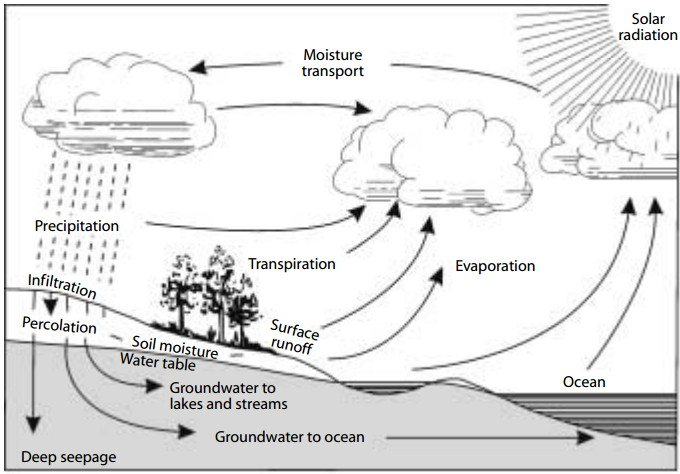
\includegraphics[width=.85\linewidth]{gfx/hydrocycle}
\end{center}
\caption{The hydrological cycle\citep{Zhang2002}. Reprinted from ``Water balance modelling: concepts and applications'', by \citeauthor{Zhang2002}, 2007, \emph{ACIAR MONOGRAPH SERIES, 84}, p.33. Copyright 2002 by \citeauthor{Zhang2002}.  }
\label{fig:hydrocycle}
\end{figure}
\newline
A variety of water balance models that derived from \autoref{eq:generalwaterbalance} exists, it can have different levels of complexity depending on the objectives of the study and data availability. 
\section{Simple bucket model}
Simple bucket model is a widely-used water balance model in a simple conceptual scenario. It considers the controlled volume system as a bucket which is filled up from rainfall and emptied by evapotranspiration. If the bucket is full, extra water added is considered deep drainage. The only data that are necessary for this model are precipitation, evaporation, transpiration and the water storage capacity of the volume. 
\section{Root zone water balance}
 The water balance model can also be applied in relatively small scaled field studies based on a specific root zone soil water balance equation \citep{Ma2013}, given as:
\begin{align}
(\theta_t - \theta_{t-1})H &= P+I-D-ET-R\label{eq:rootzonewaterbalance}
\end{align}
\begin{quote}
Where \\
$\theta_t$ and $\theta_{t-1}$ are the initial and final depth-averaged soil water content of the root zone in one time step. \\
$H$ is the root zone depth.\\
$P$ is the precipitation.\\
$I$ is the Irrigation.\\
$D$ is the drainage out of the root zone, the positive value of D means downward percolation out of the root zone, whereas the negative value of it indicates upward capillary rise into the root zone.\\ $ET$ is the actual evapotranspiration.\\
$R$ is the surface runoff. 
\end{quote}
\autoref{fig:catchment} shows the relation of a root zone modelled by the root zone water balance \autoref{eq:rootzonewaterbalance} as a plot-sized profile in a catchment. The catchment can be considered as a collection of such root zone profiles, of which the total recharge in the catchment is estimated by adding the recharge from each profile. \\
\begin{figure}[bth]
\begin{center}
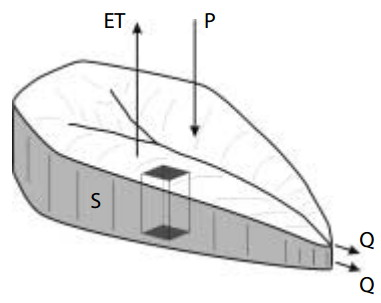
\includegraphics[width=0.5\linewidth]{gfx/catchment}
\caption{Schematic diagram of a catchment\citep{Zhang2002}. The box indicates the control volume of a root zone. S is water balance, ET is evapotranspiration, P is precipitation, Q is water runoff or flow. Reprinted from ``Water balance modelling: concepts and applications'', by \citeauthor{Zhang2002}, 2007, \emph{ACIAR MONOGRAPH SERIES, 84}, p.36. Copyright 2002 by \citeauthor{Zhang2002}. }\label{fig:catchment}
\end{center}
\end{figure}
\newline
This generalisation from root zone model is not applicable to catchments that contain complex lateral redistribution of water, thus it is difficult to estimate the recharge at a catchment scale. In most cases, it is inappropriate to assume that the catchment-scale recharge is equal to the sum of plot-scale water balance recharges, without in-depth research of the hydrogeological condition of the catchment, such as the recharge pathways and spatial heterogeneity of soil properties\citep{Zhang2002}.
 
\section{Complex models}
There are complex models that investigate not only the soil moisture dynamics but also the overall hydrological cycle over a large region of interest, they are designed to simulate interactions of different components within the system and to provide more thorough experimental results of many aspects\citep{Zhang2001}. For some purposes, simple bucket water balance models are appropriate, but other uses require greater functionality and/or more extensive analysis on a large geographic scale. For example, when analyzing the ecosystem of a large area of interest, there are various feedback between processes and different sub-systems that need to be taken into account, including the hydrological cycle, nutrient balance of soil and vegetation, heat balance, atmospheric change and more.
\subsection{Study of Amazon Basin: a system in equilibrium}
For instance, the Water Balance Model can be applied to the entire Amazon Basin in Brazil, South America  \citep{Salati1984a}, which explains the status of water flow in the Amazon forest ecosystem in a quantitative manner, as shown in \autoref{fig:amazonWaterBalance}. \\
\begin{figure}[bth]
\begin{center}
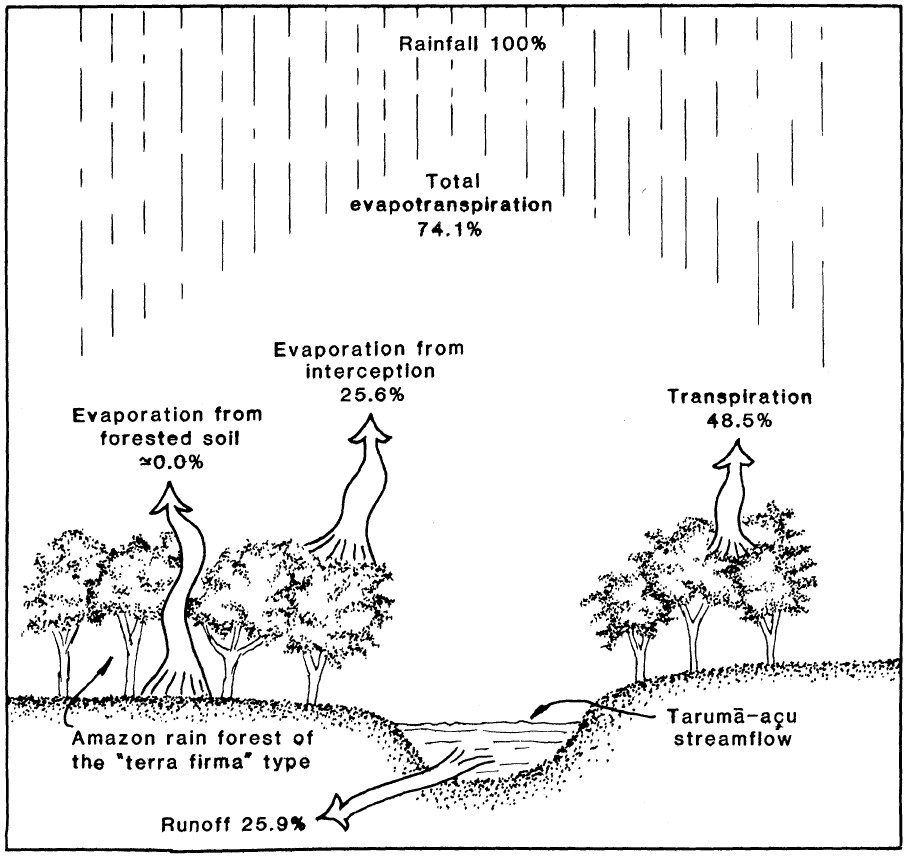
\includegraphics[width=.75\linewidth]{gfx/amazonWaterBalance}
\end{center}
\caption{Water balance from a study of a model basin near Manaus, Brazil\citep{Leopoldo1982}. Reprinted from ``Amazon basin: a system in equilibrium'', by \citeauthor{Salati1984a}, 1984, \emph{Science,4658}, p.130. Copyright 1984 by \citeauthor{Salati1984a}.  }
\label{fig:amazonWaterBalance}
\end{figure}
\newline
This model applies to the horseshoe-shaped Amazon Basin as a whole system, it uses knowledge of different domains in Meteorology. However, due to the lack of proper infrastructure in Brazil when the study was conducted. Accurate measurements on precipitation, evapotranspiration and other hydrological attributes over a large area were not available for analysis at a high precision level. \\
\newline
The measurements were taken from 1981 to 1983 in a controlled field in Barro-Branco watershed\citep{Leopoldo1995}. Precipitation data was obtained by use of a simple rain gauge installed at the reserve's meteorological station whereas the discharge was determined by use of a 0.8-m-wide rectangular weir and a water level recorder. Thus, the inferences of the influx and efflux of water in the area are based on assumptions made from wind conditions and a single point-based data as the averaged value over large areas which includes non-forest areas and are also influenced by other factors. 

\section{Water Balance Model for this Thesis}
There is a trade-off in choosing between complex models and simpler models such as the simple bucket model for conducting the analysis in this thesis. With greater functionality comes greater complexity. One of the issues with using a more complex water balance model is that there are more parameters required to complete the model. Which means that more data and man-hours are involved to understand and interpret the equation into a machine-readable form. If there isn't sufficient data of various parameters, then selecting a complex model is inappropriate for the objectives. The key to successful modelling is to match model complexity with data availability and the analysis objectives.
\subsection{Data availability}\label{subsection:dataavailability}
The objective of analysis in this thesis primarily concentrates on Australia as opposed to any other regions. Thus, one of the main data source being used is the Australian Water Availability Project (AWAP), which provides historic temporal-spatial meteorology data for the entire Australia. As described in the AWAP Final Report \citep{Raupach2009}, the AWAP is a partnership between CSIRO Marine and Atmospheric Research (CMAR), the Bureau of Meteorology (BoM) and the Bureau of Rural Science (BRS), aiming to monitor the status and trend of the water balance of the Australian territories, using model-data fusion methods to combine measurements and model predictions. The AWAP data is discussed in more detail in \autoref{ch:dataintegration} \nameref{ch:dataintegration}.\\
\newline
The AWAP provides essential meteorology data for water balance calculations, such as the precipitation, evapotranspiration, surface runoff and deep drainage etc.\\
\newline
A farm location in Richmond, Tasmania, Australia, of geographic coordinate latitude: -42.61 and longitude: 147.39, is chosen for demonstration purpose. The location is marked on Google Maps\citep{Google2014} as shown in \autoref{fig:gmapexample}.\\
\begin{figure}[hbt]
\begin{center}
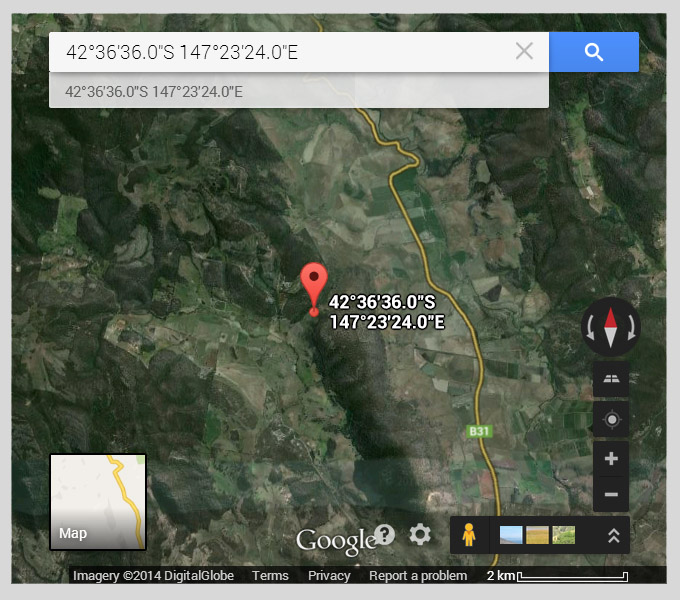
\includegraphics[width=0.75\linewidth]{gfx/gmapexample}
\end{center}
\caption{Satellite View of location latitude: -42.61 and longitude: 147.39, in Tasmania, Australia. Acquired from Google Maps.}
\label{fig:gmapexample}
\end{figure}
\newline
For this given location, the following time-series data of meteorology attributes: precipitation, evapotranspiration of soil and vegetation, open water evapotranspiration, surface runoff and deep drainage are acquired from AWAP, plotted in \autoref{fig:raints}, \autoref{fig:evapts}, \autoref{fig:surfrunts} and \autoref{fig:deepdraints} respectively. \\
\begin{figure}[hbt]
\begin{center}
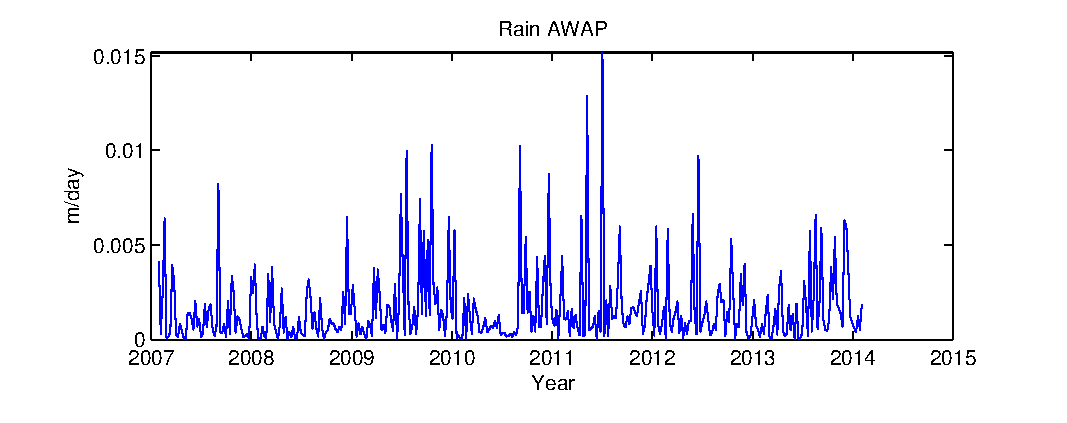
\includegraphics[width=\linewidth]{gfx/raints.eps}
\end{center}
\caption{Time series of AWAP data: Rainfall, for location lat: -42.61, lon:147.39}
\label{fig:raints}
\end{figure}
\newline
\autoref{fig:raints} shows the rainfall data of this location, plotted from Year 2007 to 2014. It has shown a consistent amount of precipitation for each of the years. The maximum rainfall per day is 0.0152 m/day which occurred during the week of 04-Jul-2011. Furthermore, year 2011-2012 has a slightly higher overall precipitation amount than the other years. In general, the chosen location has a dry start, then wet in Summer and Autumn throughout the year\citep{tasmania2013}. \\
\begin{figure}[hbt]
\begin{center}
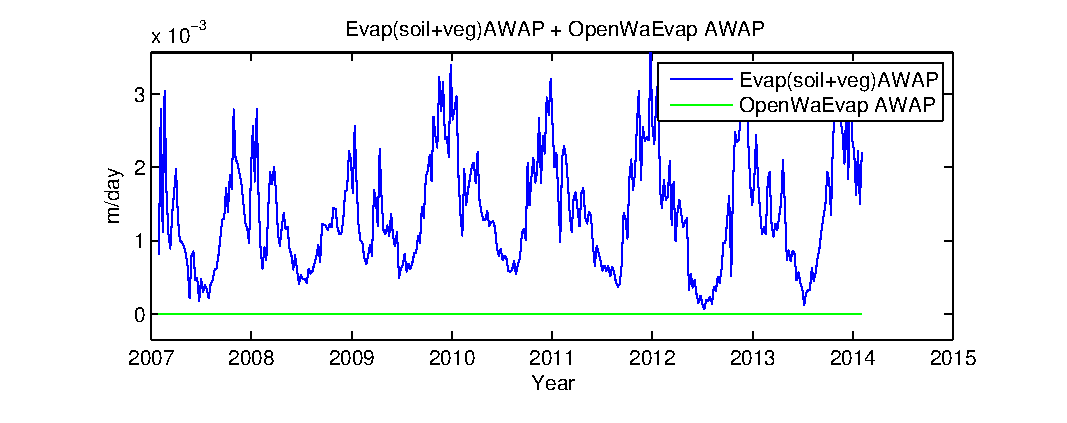
\includegraphics[width=\linewidth]{gfx/evapts.eps}
\end{center}
\caption{Time series of AWAP data: Evapotranspiration of soil and vegetation, and Open water evapotranspiration, for location lat: -42.61, lon:147.39}
\label{fig:evapts}
\end{figure}
\newline
\autoref{fig:evapts} shows the evapotranspiration data of this location. The blue line indicates the combined evapotranspiration of soil and vegetation, which has a clear and consistent chronological pattern throughout the years. The evapotranspiration reaches its lowest point during Winter season and climbs up to the highest point in the Summer season, which then declines during Autumn thus forming a repetition pattern. \\
On the other hand, open water evapotranspiration is indicated by the green line, which remains as zero for this location, due to the lack of open water in the surrounding terrestrial environment.\\
\begin{figure}[hbt]
\begin{center}
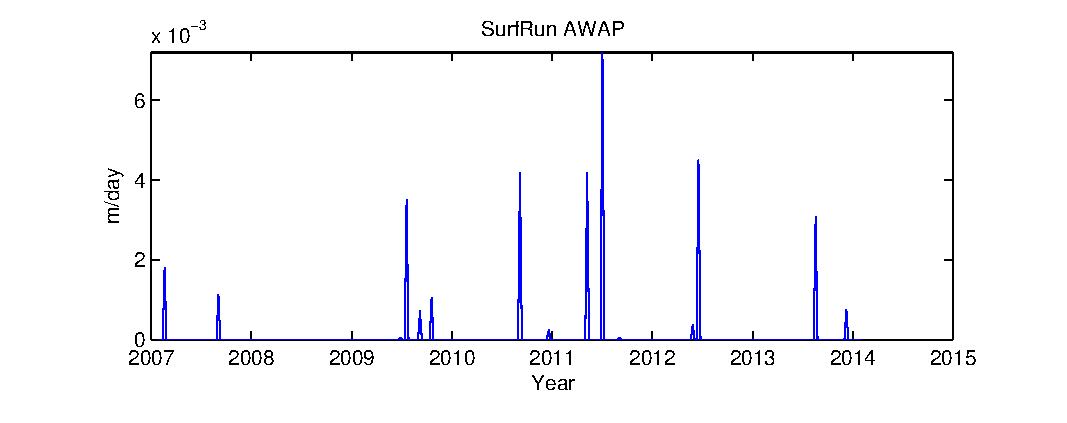
\includegraphics[width=\linewidth]{gfx/surfrunts.eps}
\end{center}
\caption{Time series of AWAP data: Surface Runoff, for location lat: -42.61, lon:147.39}
\label{fig:surfrunts}
\end{figure}
\newline
\autoref{fig:surfrunts} shows the surface runoff data of this location. Throughout the timespan, most of the weeks' surface runoff are zero while there are a few spikes in the figure. According to the AWAP datasheet\citep{Raupach2009}:
\begin{quote}
\emph{Surface runoff (FWRun) is given by a step function: all precipitation runs off when the upper-layer soil is saturated, and there is no runoff otherwise.}
\end{quote}
\begin{figure}[hbt]
\begin{center}
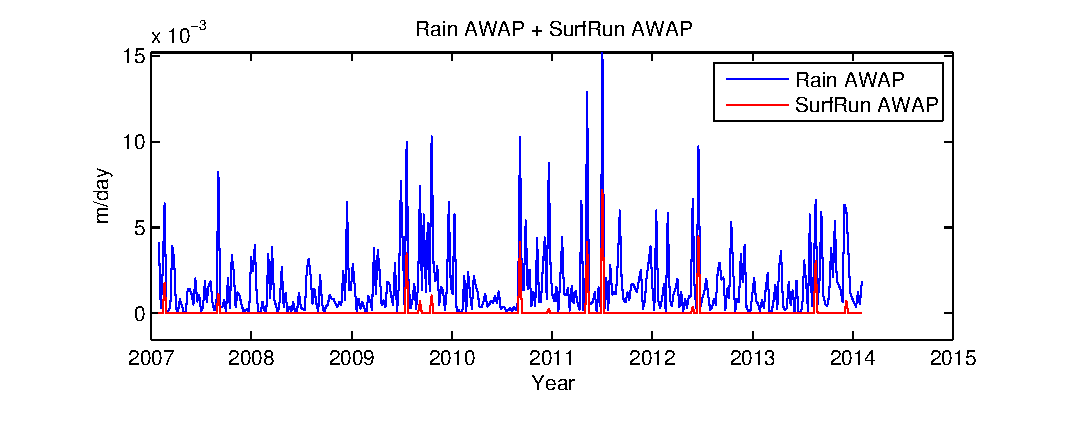
\includegraphics[width=\linewidth]{gfx/rainsurfts.eps}
\end{center}
\caption{Time series of AWAP data: Rainfall and Surface Runoff, for location lat: -42.61, lon:147.39}
\label{fig:rainsurfts}
\end{figure}
As shown in \autoref{fig:rainsurfts}, by comparing the rainfall data, as indicated by the blue line, and the surface runoff data, as indicated by the red line, we can confirm that the above statement is correct, because the spikes of surface runoff only occur where there are continuously heavier rainfalls. That is, surface water runoff occur only when the soil moisture is in saturation status due to heavy and continuous precipitation.\\
\begin{figure}[hbt]
\begin{center}
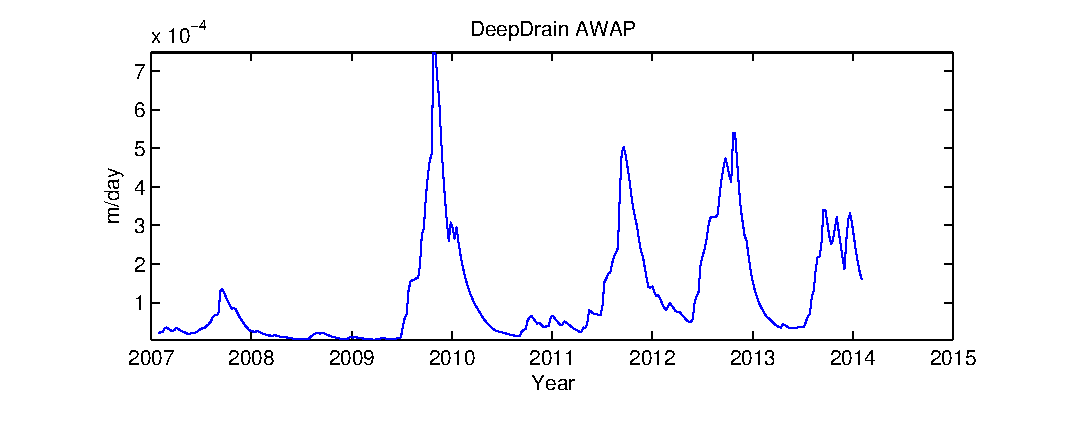
\includegraphics[width=\linewidth]{gfx/deepdraints.eps}
\end{center}
\caption{Time series of AWAP data: Deep Drainage, for location lat: -42.61, lon:147.39}
\label{fig:deepdraints}
\end{figure}
\newline
\autoref{fig:deepdraints} shows the deep drainage data of this location. By observing the curve itself, there is not any linear or chronological pattern apparent in the data. Nevertheless, according to the AWAP datasheet:
\begin{quote}\begin{minipage}{0.9\textwidth}
\emph{Leaching ($F_{\text{WLch}}$) or drainage downward out of soil layer i is given by}
\begin{align}
F_{\text{WLch}~i} &= K_{Si}w_i^\gamma
\label{eq:awapleaching}
\end{align}
\emph{Where $\gamma$ is an exponent specifying the response of drainage to relative soil water $w_i$, and $K_{Si}$ [m/day] is the saturated hydraulic conductivity of soil layer i.}
\end{minipage}\end{quote}
\begin{figure}[hbt]
\begin{center}
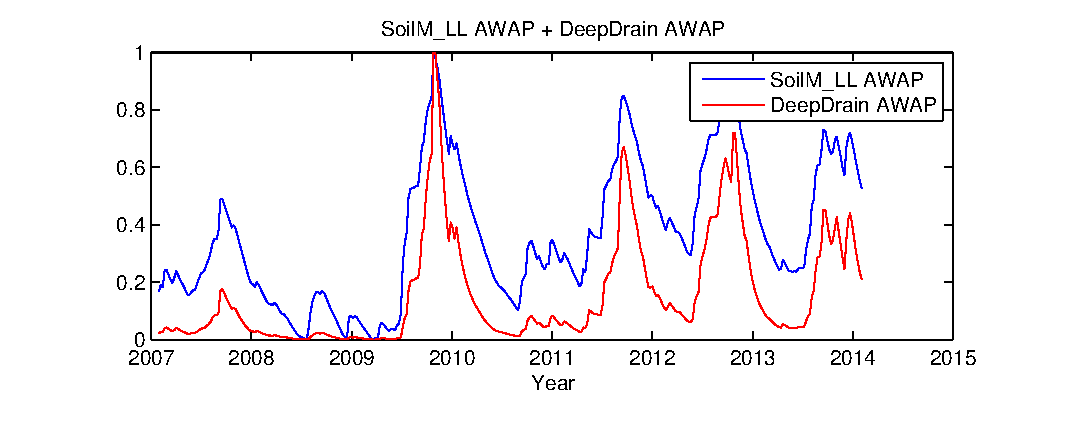
\includegraphics[width=\linewidth]{gfx/soilmdeepts.eps}
\end{center}
\caption{Time series of normalized AWAP data: Deep Drainage and Soil Moisture of low level, for location lat: -42.61, lon:147.39}
\label{fig:soilmdeepts}
\end{figure}
\autoref{fig:soilmdeepts} plots the soil moisture of low level and normalized deep drainage on the same figure. The data are normalized against the minimum and maximum so that both data scale from 0 to 1. There is an apparent direct correlation between the two meteorological attributes of the point of interest, which confirms the relationship defined in \autoref{eq:awapleaching}. This means that deep drainage occur if the lower level of soil moisture is saturated.
\subsection{Implementing water balance model}
In this thesis, a water balance model is implemented from the equation 
\begin{align}
	\Delta \langle S\rangle &= \langle P\rangle - \langle ET\rangle-\langle Q\rangle-\langle R\rangle
	\label{eq:wbsimple}
\end{align}
\begin{quote}Where \\
\indent$\Delta \langle S\rangle$ is the change in spatially averaged catchment water storage, which ideally is zero when there is perfect balanced influx and efflux of the system.\\
\indent$\langle P\rangle$ is the spatially averaged precipitation, acquired from AWAP rainfall data, represented by the variable \emph{\{rain AWAP\}} in the integrated data source.\\
\indent$\langle ET\rangle$ is the spatially averaged catchment evapotranspiration, acquired by adding two variables from AWAP, evapotranspiration of soil and vegetation \& open water evapotranspiration, represented in the integrated data source as \emph{\{Evap(soil+veg)AWAP + OpenWaEvap AWAP\}}.\\
\indent$\langle Q\rangle$ is the spatially averaged catchment surface runoff, acquired from AWAP surface runoff data, represented by the variable \emph{\{SurfRun AWAP\}}.\\
\indent$\langle R\rangle$ is the spatially averaged catchment recharge, acquired from AWAP deep drainage data, represented by the variable \emph{\{DeepDrain AWAP\}}, while sub-surface flow is considered zero.
\end{quote}
\begin{figure}[hbt]
\begin{center}
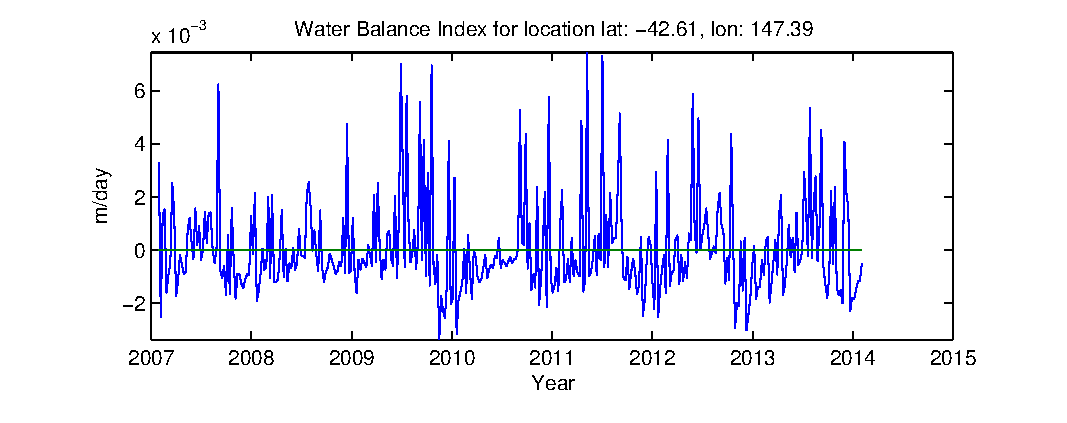
\includegraphics[width=\linewidth]{gfx/waterts.eps}
\end{center}
\caption{Time series of calculated water balance index from AWAP data, for location lat: -42.61 lon:147.39}
\label{fig:waterts}
\end{figure}
\autoref{fig:waterts} plots the calculated water balance index for the given location from year 2007 to 2014, using \autoref{eq:wbsimple}. For this point of interest, the water balance index fluctuates around the zero line, which means during the time when there is rainfall, the water balance is at higher level, and vice versa.\\
\begin{figure}[hbt]
\begin{center}
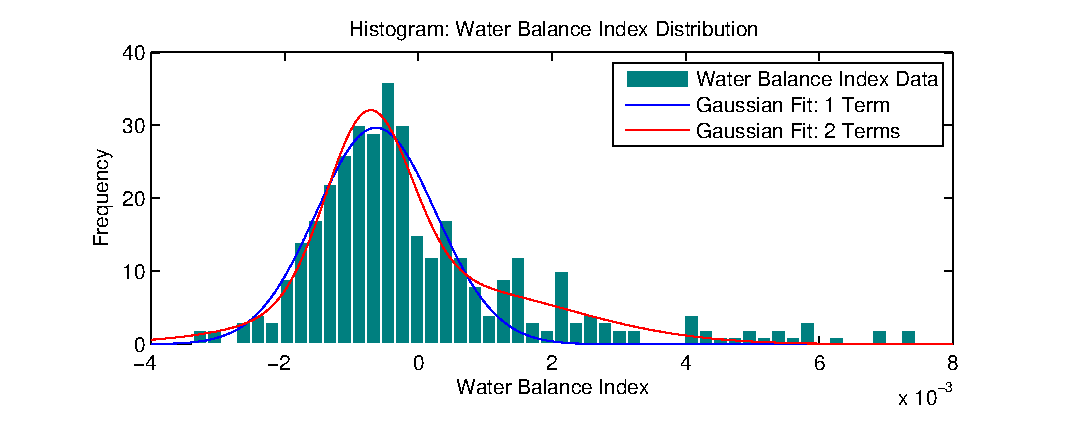
\includegraphics[width=\linewidth]{gfx/waterhist.eps}
\end{center}
\caption{Histogram of calculated water balance index with fitted Gaussian Distribution}
\label{fig:waterhist}
\end{figure}
\newline
The histogram of the water balance index data is plotted with 50 bars, as shown in \autoref{fig:waterhist}. Two Gaussian distributions are generated to fit the data, both one term and two terms fittings, the parameters are given below.\graffito{{\color{red}Explain the physical meaning of having normally distributed water balance indices.}}
\begin{quote}
\begin{align}
f(x)&=a_1*e^{-((x-b_1)/c_1)^2)}\label{eq:gaussianfit1}\\
g(x)&=a_2*e^{-((x-b_2)/c_2)^2)}+a_3*e^{-((x-b_2)/c_2)^2)}
\end{align}
Where the coefficients (with 95\% confidence bounds) are:\\
$a_1 = 29.68~(26.58, 32.78)\\
b_1 =  -0.0006337~ (-0.0007418, -0.0005256)\\
c_1 =    0.001269  ~(0.001116, 0.001422)\\
a_2 =       25.25 ~ (20.61, 29.89)\\
       b_2 =  -0.0007439 ~ (-0.0008451, -0.0006426)\\
       c_2 =   0.0008972  ~(0.000711, 0.001083)\\
       a_3 =       7.916  ~(4.042, 11.79)\\
       b_3 =   0.0003042~  (-0.00053, 0.001138)\\
       c_3 =    0.002693  ~(0.001877, 0.00351)$
\end{quote}
From the Gaussian distribution fittings in \autoref{fig:waterhist}, the data generally is normally distributed while slightly skewed to the right. 
 % Chapter 2
% Chapter 3

\chapter{Data Integration} % Chapter title

\label{ch:dataintegration} % For referencing the chapter elsewhere, use \autoref{ch:mathtest}
%----------------------------------------------------------------------------------------
%
%----------------------------------------------------------------------------------------
\section{The Datasets}
\subsection{Australian Water Availability Project}
As mentioned in \autoref{subsection:dataavailability} \nameref{subsection:dataavailability}, the Australian Water Availability Project (AWAP) is a joint effort contributed by CSIRO Marine and Atmospheric Research (CMAR), the Bureau of Meteorology (BoM) and the Bureau of Rural Science (BRS)\citep{Raupach2009}.\\
\newline
The AWAP aims to contribute to the overall understanding and monitoring of the Australian landscape systems, particularly the changes and feedback in climate, so that proper and robust management can be applied on a system-scale. It monitors the state and trend of the terrestrial water balance of the Australian continent.\\
\newline 
The approach it takes is based on model-data fusion, which is combining information from both the models and the data to maximise knowledge about the system. It contains historic and up-to-date data of soil moisture and all water influx and efflux contributing to changes in soil moisture (rainfall, transpiration, soil evaporation, surface runoff and deep drainage etc.), across Australia at a spatial resolution of 5 km. \\
\newline 
The AWAP data is available for access through a web interface, it provides three forms: (1) weekly near-real-time reporting, (2) historical monthly time series (1900 to present), and (3) monthly climatologies.\\
\begin{figure}[hbt]
\myfloatalign
\subfloat[{Precipitaion[mm/d]}]
{\label{fig:awapprec1}
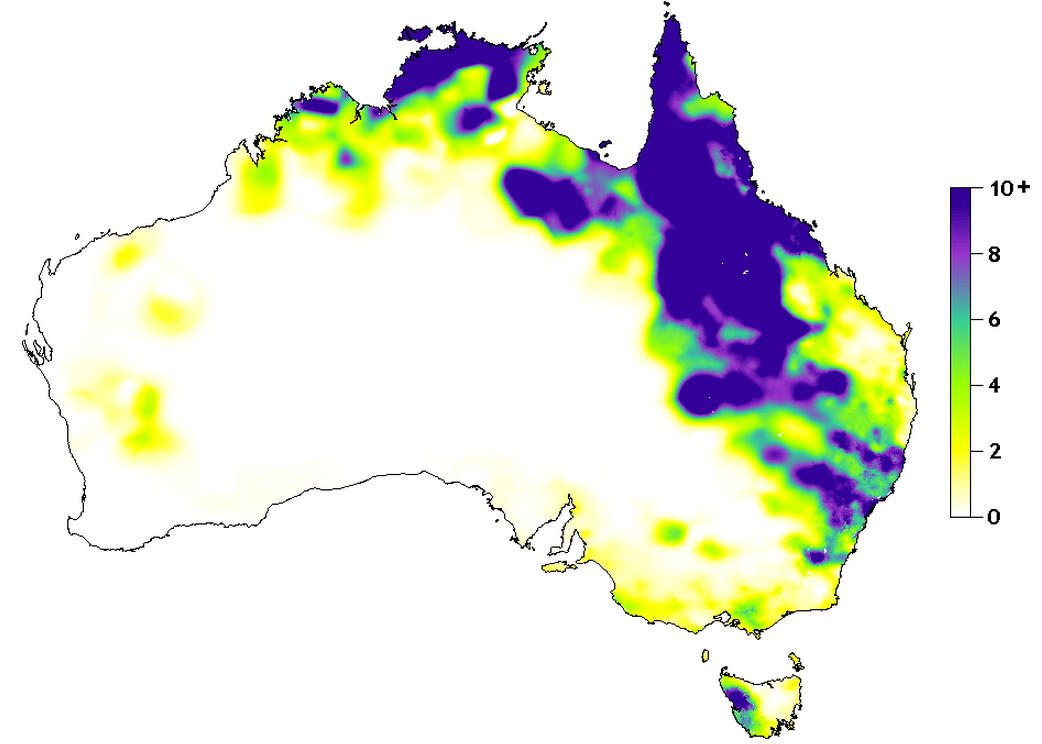
\includegraphics[width=.45\linewidth]{gfx/awapprec}} \quad
\subfloat[{Percent Rank Precipitaion[\%]}]
{\label{fig:awapprec2}
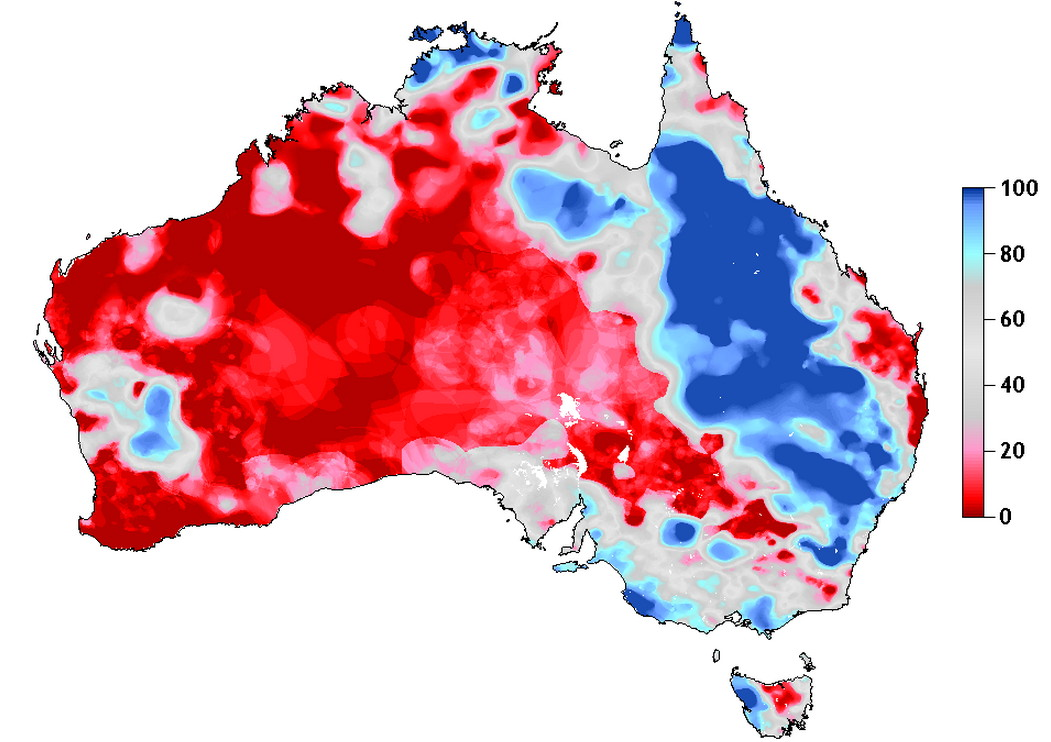
\includegraphics[width=.45\linewidth]{gfx/awapprecper}}
\caption{Example of AWAP weekly near-real-time data. Date: 2014/02/17 to 2014/02/23. Acquired from CSIRO\citep{Awap2014}.}
\label{fig:awapprec}
\end{figure}
\newline
\autoref{fig:awapprec} shows an example of AWAP weekly data acquired from the web interface hosted by CSIRO. The example displays the precipitaion data in both physical values(\autoref{fig:awapprec1}) and percentage rank(\autoref{fig:awapprec2}) of the week from 2014/02/17 to 2014/02/23 on the Australian territories.
\subsection{CosmOz: Australian National Cosmic Ray Soil Moisture Monitoring Facility} 
The Australian National Cosmic Ray Soil Moisture Monitoring Facility(CosmOz) is a near-real-time soil moisture measurement network provided by CSIRO, Monash University, Charles Darwin University and the University of New South Wales\citep{cosmoz2014}. it aims to test the utility of cosmic ray sensor system for water management, water information and hydrological process research applications, as well as to test the feasibility and utility of a national near-real time soil moisture measurement network. CosmOz also supports the evaluation of remote sensing products and hydrological models by expanding the set of soil moisture data available over Australia.\\
\newline
CosmOz currently has deployed 13 sensor systems at 12 locations across Australia, shown in \autoref{fig:cosmozloc}. Each CosmOz sensor system includes: 1* Hydroinnova CRS-1000 cosmic ray soil moisture sensor, 1* Hydrological Services tipping-bucket rain gauge, 3* Campbell TDR soil moisture probes and Quaesta data logger with integrated Iridium SBS satellite data communications.
\begin{figure}[hbt]
\myfloatalign
\subfloat[{Location of the 12 CosmOz monitoring sites. Acquired from University of Arizona\citep{arizona2014}}]
{\label{fig:cosmozloc}
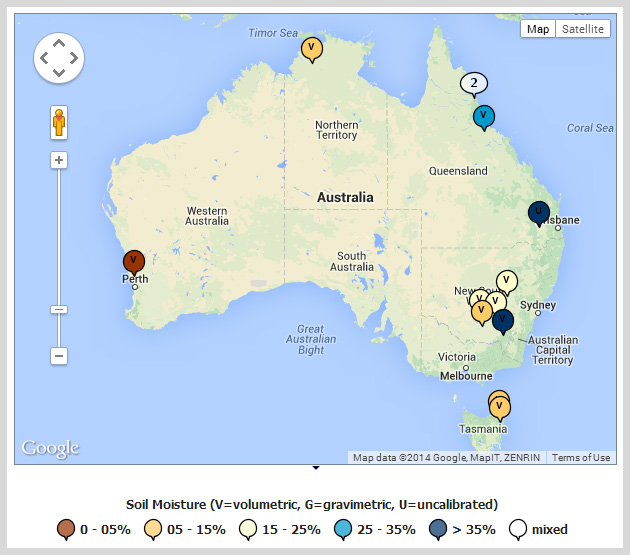
\includegraphics[width=.52\linewidth]{gfx/cosmozloc}} \quad
\subfloat[{CosmOz system installed at Tullochgorum in Tasmania. Reprinted from ``{C}osm{O}z {W}iki Page'', by \citeauthor{cosmoz2014}, 2013. Copyright 2013 by \citeauthor{cosmoz2014}.}]
{\label{fig:cosmozphoto}
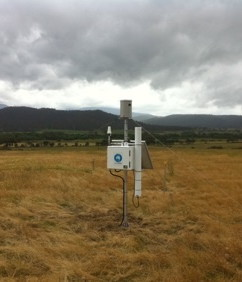
\includegraphics[width=.39\linewidth]{gfx/cosmozphoto}}
\caption{The Australian National Cosmic Ray Soil Moisture Monitoring Facility(CosmOz) and one of its probes deployed in Tullochgorum site.}
\label{fig:cosmoz}
\end{figure}

\subsection{Landsat program}
The Landsat program is a joint effort of the U.S. Geological Survey (USGS) and the National Aeronautics and Space Administration (NASA). The lantsat satellites have continuously acquired and delivered images of the Earth's land surface since 1972\citep{Mission2013}. The Landsat satellites have provided a valuable archive of space-based land remotely sensed data, contributed greatly in the studies of agriculture, geology, forestry, education, region planning, mapping and global change research.\\
\begin{figure}[bth]
\begin{center}
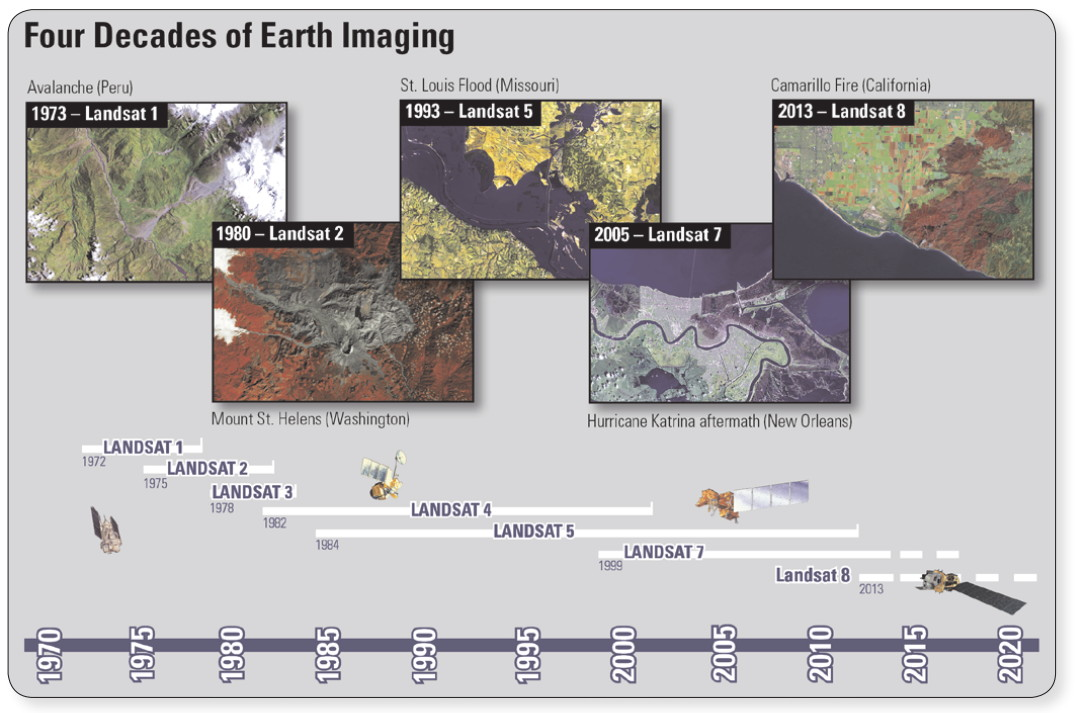
\includegraphics[width=.95\linewidth]{gfx/landsat}
\end{center}
\caption{Overview of the Landsat program. Reprinted from ``Landsat: A Global Land-Imaging Mission'', by USGS, 2013. Copyright 2013 by USGS.  }
\label{fig:landsat4decades}
\end{figure}
\newline
Landsat 8 is the eighth and the latest Landsat satellite, launched on 11 February 2013. \autoref{table:landsatsum} details the eight Landsat satellites in terms of launch/decommission time, operation status and the sensors on-board respectively. In the ``Sensors'' column, Landsat 1,2,3 carries Multispectral Scanner (MSS) and Return Beam Vidicon Camera (RBV), Landsat 4,5 carries MSS and Thematic Mapper (TM), Landsat 6 carries Enhanced Thematic Mapper (ETM), Landsat 7 carries Enhanced Thematic Mapper Plus (ETM+) and Landsat 8 carries Operational Land Imager (OLI) and Thermal Infrared Sensor (TIRS).\\
\begin{table}[hbt]
\caption{Details of Landsat missions. Adapted from ``Landsat: A Global Land-Imaging Mission'', by USGS, 2013. Copyright 2013 by USGS.}
\begin{center}
\rowcolors{2}{cyan!15}{white} 
\begin{tabular}{llll} 
\hline
\textbf{Satellite}&\textbf{Launch}&\textbf{Decommissioned}&\textbf{Sensors}\\
\hline
Landsat 1 & 23 July 1973 & 6 January 1978 & MSS/RBV \\
Landsat 2 & 22 January 1975 & 27 July 1983 & MSS/RBV \\
Landsat 3 & 5 March 1978 & 7 Septermber 1983 & MSS/RBV \\
Landsat 4 & 16 July 1982 & 15 July 2001 & MSS/TM \\
Landsat 5 & 1 March 1984 & 2013 & MSS/TM \\
Landsat 6 & 5 October 1993 & Did not achieve orbit & ETM\\
Landsat 7 & 15 April 1999 & Operational & ETM+ \\
Landsat 8 & 11 February 2013 & Operational & OLI/TIRS\\
\hline 
\end{tabular}
\end{center}
\label{table:landsatsum}
\end{table}
\newline
It is noteworthy that both Landsat 6 and Landsat 7 suffered from operational failures. Landsat 6 did not achieve its target orbit during launching procedure, thus it was officially declared as a failure by the National Oceanic and Atmospheric Administration (NOAA)\citep{Viets1995}. Landsat 7 experienced a failure in its Scan Line Corrector (SLC) mechanism, which resulted in wedge-shaped scan-to-scan gaps. As shown in \autoref{fig:l7slcoff} comparing to \autoref{fig:l7slcon}, there are blank gaps on the image where data is not available.
\begin{figure}[hbt]
\myfloatalign
\subfloat[{Landsat 7 Natural Color Image with SLC-ON. Captured on 9 January 2003.}]
{\label{fig:l7slcon}
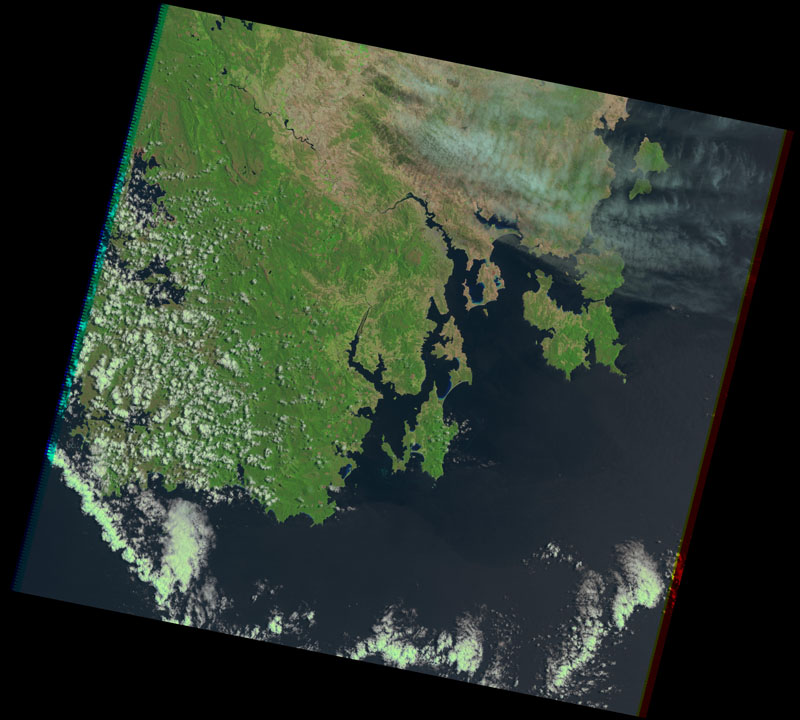
\includegraphics[width=.45\linewidth]{gfx/l7slcon}} \quad
\subfloat[{Landsat 7 Natural Color Image with SLC-OFF (with gaps). Captured on 25 March 2007.}] 
{\label{fig:l7slcoff}
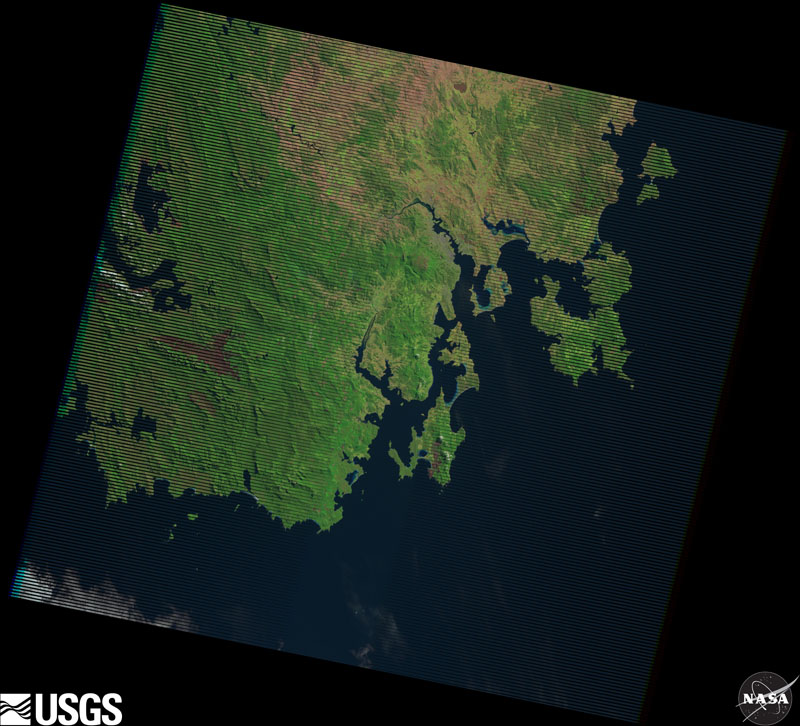
\includegraphics[width=.45\linewidth]{gfx/l7slcoff}}
\caption{Landsat 7 ETM+ images of the Tasmania south-eastern area captured before and after the SLC failure. Acquired from USGS.}
\label{fig:l7slc}
\end{figure}

\subsection{Moderate-resolution Imaging Spectroradiometer}

\subsection{National Elevation Data Framework}

\subsection{SILO}

 % Chapter 3
% Chapter X

\chapter{Chapter Title} % Chapter title

\label{ch:name} % For referencing the chapter elsewhere, use \autoref{ch:name} 

%----------------------------------------------------------------------------------------

\section{Section Title}

Content

%------------------------------------------------

\subsection{Subsection Title}

Content

%------------------------------------------------

\subsection{Subsection Title}

Content

%----------------------------------------------------------------------------------------

\section{Section Title}

Content % Chapter 4
% Chapter 5

\chapter{Conclusions} % Chapter title

\label{ch:conclusion} % For referencing the chapter elsewhere, use \autoref{ch:name} 

%----------------------------------------------------------------------------------------
\section{Summary of work}
For the work outlined in the previous chapters in the thesis, a total count of 50 classes of 12 Java packages were implemented for the system which sums up to an approximate of 8,000 lines of code exclusive of blank lines. On top of that, a total number of 23 MATLAB scripts have been produced for the analytical work which include both the first stage point-based analysis using D-LDA method and the second stage area-wise multivariate analysis of the integrated knowledge base. In addition, a user manual for the java package \emph{au.csiro.iekbase.integration} has been written and formally typesetted for giving instructions on how to set up a knowledge base for any arbitrary location within Australia. The implementation and analytical results for the first stage work of the thesis has been published on peer-reviewed journal and presented in an IEEE Conference in Baltimore, MD, USA in November 2013\citep{Li2013}. The work carried out for the second stage analysis has novelties in regards to the approach it undertook for the water balance evaluation on a continental scale, of which the manuscript of a journal article has been drafted and due for peer-review and publication in the near future.
\section{Further development}
To extend from the work completed in the thesis, firstly, a further set of supervised machine learning algorithms can be trialed on the data set, potentially includes but not limited to \acp{hmm} which has proven effective especially for time series data and a few other neutral networks. Secondly, the current weekly directory structure of the integrated knowledge base has a flaw in its design which is that in the case where the a small portion of the data for analysis is required, for example, one variable of the AWAP data, such as the rainfall of a given location is needed, the entire data file needs to be loaded completely for the content to be extracted.  Also, modifications to the location of a defined case study is inefficient in the sense that a complete rerun needs to be performed for such alteration to take place.\\
\newline
A \ac{gui} can be developed in a similar manner that was employed for the point-based proof-of-concept demo, for the area-wise analysis to provide an easy-to-use digital platform for the farming practitioners to utilise thus fulfilling the initial objective as a irrigation water usage decision support system.\\
\newline
The proposed approach for heterogeneous knowledge integration in the thesis can be applied to fields of research other than water balance estimation which was the main focus of the outlined work. Given sufficient data of various independent data sources, it is theoretically viable to attempt to use one widely available input in terms of spatial and temporal resolutions as a proxy to an environmental attribute that is conventionally measured via field experimentation or empirical modelling, thus overcoming the drawbacks of having limited experimental results over a long timespan due to practical difficulties and/or financial constraints etc. Examples of such studies could include but not limited to: the human impact on the Great Barrier Reef ecosystem - a continuous study of human behaviour to the environment; the deforestation of the Amazon tropical forest in the South America - Is there a specific human-factor involved or it is merely a process of the Earth ecosystem's natural cycle. % Chapter 5

%----------------------------------------------------------------------------------------
%	THESIS CONTENT - APPENDICES
%----------------------------------------------------------------------------------------
 
\appendix

% Appendix A

\chapter{Appendix Test}

%----------------------------------------------------------------------------------------

\lipsum[13-14]

%----------------------------------------------------------------------------------------

\section{Appendix Section Test}
\lipsum[15]

\graffito{More dummy text}
\lipsum[16]

%----------------------------------------------------------------------------------------

\section{Another Appendix Section Test}
\lipsum[17]

\begin{table}
\myfloatalign
\begin{tabularx}{\textwidth}{Xll} \toprule
\tableheadline{labitur bonorum pri no} & \tableheadline{que vista}
& \tableheadline{human} \\ \midrule
fastidii ea ius & germano &  demonstratea \\
suscipit instructior & titulo & personas \\
\midrule
quaestio philosophia & facto & demonstrated \\
\bottomrule
\end{tabularx}
\caption[Autem usu id]{Autem usu id.}
\label{tab:moreexample}
\end{table}

\lipsum[18]

\begin{lstlisting}[float,caption=A floating example]
for i:=maxint to 0 do
begin
{ do nothing }
end;
\end{lstlisting} % Appendix A
%% Appendix X

\chapter{Appendix Title}

%----------------------------------------------------------------------------------------

% Content begins here % Appendix B - empty template
 
%----------------------------------------------------------------------------------------
%	POST-CONTENT THESIS PAGES
%----------------------------------------------------------------------------------------

\cleardoublepage% Bibliography

\label{app:bibliography} % Reference the bibliography elsewhere with \autoref{app:bibliography}

\manualmark
\markboth{\spacedlowsmallcaps{\bibname}}{\spacedlowsmallcaps{\bibname}} 
\refstepcounter{dummy}

\addtocontents{toc}{\protect\vspace{\beforebibskip}} % Place the bibliography slightly below the rest of the document content in the table of contents
\addcontentsline{toc}{chapter}{\tocEntry{\bibname}}

\bibliographystyle{unsrtnat}

\bibliography{Bibliography,manual} % Bibliography

%\cleardoublepage% Colophon (a brief description of publication or production notes relevant to the edition)

\pagestyle{empty}

\hfill

\vfill

\pdfbookmark[0]{Colophon}{colophon}

\section*{Colophon}

This document was typeset using the typographical look-and-feel \texttt{classicthesis} developed by Andr\'e Miede. The style was inspired by Robert Bringhurst's seminal book on typography ``\emph{The Elements of Typographic Style}''. \texttt{classicthesis} is available for both \LaTeX\ and \mLyX: 

\begin{center}
\url{http://code.google.com/p/classicthesis/}
\end{center}

\noindent Happy users of \texttt{classicthesis} usually send a real postcard to the author, a collection of postcards received so far is featured here: 

\begin{center}
\url{http://postcards.miede.de/}
\end{center}
 
\bigskip

\noindent\finalVersionString % Colophon


%----------------------------------------------------------------------------------------

\end{document}
